% Options for packages loaded elsewhere
\PassOptionsToPackage{unicode}{hyperref}
\PassOptionsToPackage{hyphens}{url}
\documentclass[
  ignorenonframetext,
]{beamer}
\newif\ifbibliography
\usepackage{pgfpages}
\setbeamertemplate{caption}[numbered]
\setbeamertemplate{caption label separator}{: }
\setbeamercolor{caption name}{fg=normal text.fg}
\beamertemplatenavigationsymbolsempty
% remove section numbering
\setbeamertemplate{part page}{
  \centering
  \begin{beamercolorbox}[sep=16pt,center]{part title}
    \usebeamerfont{part title}\insertpart\par
  \end{beamercolorbox}
}
\setbeamertemplate{section page}{
  \centering
  \begin{beamercolorbox}[sep=12pt,center]{section title}
    \usebeamerfont{section title}\insertsection\par
  \end{beamercolorbox}
}
\setbeamertemplate{subsection page}{
  \centering
  \begin{beamercolorbox}[sep=8pt,center]{subsection title}
    \usebeamerfont{subsection title}\insertsubsection\par
  \end{beamercolorbox}
}
% Prevent slide breaks in the middle of a paragraph
\widowpenalties 1 10000
\raggedbottom
\AtBeginPart{
  \frame{\partpage}
}
\AtBeginSection{
  \ifbibliography
  \else
    \frame{\sectionpage}
  \fi
}
\AtBeginSubsection{
  \frame{\subsectionpage}
}
\usepackage{iftex}
\ifPDFTeX
  \usepackage[T1]{fontenc}
  \usepackage[utf8]{inputenc}
  \usepackage{textcomp} % provide euro and other symbols
\else % if luatex or xetex
  \usepackage{unicode-math} % this also loads fontspec
  \defaultfontfeatures{Scale=MatchLowercase}
  \defaultfontfeatures[\rmfamily]{Ligatures=TeX,Scale=1}
\fi
\usepackage{lmodern}
\ifPDFTeX\else
  % xetex/luatex font selection
\fi
% Use upquote if available, for straight quotes in verbatim environments
\IfFileExists{upquote.sty}{\usepackage{upquote}}{}
\IfFileExists{microtype.sty}{% use microtype if available
  \usepackage[]{microtype}
  \UseMicrotypeSet[protrusion]{basicmath} % disable protrusion for tt fonts
}{}
\makeatletter
\@ifundefined{KOMAClassName}{% if non-KOMA class
  \IfFileExists{parskip.sty}{%
    \usepackage{parskip}
  }{% else
    \setlength{\parindent}{0pt}
    \setlength{\parskip}{6pt plus 2pt minus 1pt}}
}{% if KOMA class
  \KOMAoptions{parskip=half}}
\makeatother
\usepackage{color}
\usepackage{fancyvrb}
\newcommand{\VerbBar}{|}
\newcommand{\VERB}{\Verb[commandchars=\\\{\}]}
\DefineVerbatimEnvironment{Highlighting}{Verbatim}{commandchars=\\\{\}}
% Add ',fontsize=\small' for more characters per line
\usepackage{framed}
\definecolor{shadecolor}{RGB}{248,248,248}
\newenvironment{Shaded}{\begin{snugshade}}{\end{snugshade}}
\newcommand{\AlertTok}[1]{\textcolor[rgb]{0.94,0.16,0.16}{#1}}
\newcommand{\AnnotationTok}[1]{\textcolor[rgb]{0.56,0.35,0.01}{\textbf{\textit{#1}}}}
\newcommand{\AttributeTok}[1]{\textcolor[rgb]{0.13,0.29,0.53}{#1}}
\newcommand{\BaseNTok}[1]{\textcolor[rgb]{0.00,0.00,0.81}{#1}}
\newcommand{\BuiltInTok}[1]{#1}
\newcommand{\CharTok}[1]{\textcolor[rgb]{0.31,0.60,0.02}{#1}}
\newcommand{\CommentTok}[1]{\textcolor[rgb]{0.56,0.35,0.01}{\textit{#1}}}
\newcommand{\CommentVarTok}[1]{\textcolor[rgb]{0.56,0.35,0.01}{\textbf{\textit{#1}}}}
\newcommand{\ConstantTok}[1]{\textcolor[rgb]{0.56,0.35,0.01}{#1}}
\newcommand{\ControlFlowTok}[1]{\textcolor[rgb]{0.13,0.29,0.53}{\textbf{#1}}}
\newcommand{\DataTypeTok}[1]{\textcolor[rgb]{0.13,0.29,0.53}{#1}}
\newcommand{\DecValTok}[1]{\textcolor[rgb]{0.00,0.00,0.81}{#1}}
\newcommand{\DocumentationTok}[1]{\textcolor[rgb]{0.56,0.35,0.01}{\textbf{\textit{#1}}}}
\newcommand{\ErrorTok}[1]{\textcolor[rgb]{0.64,0.00,0.00}{\textbf{#1}}}
\newcommand{\ExtensionTok}[1]{#1}
\newcommand{\FloatTok}[1]{\textcolor[rgb]{0.00,0.00,0.81}{#1}}
\newcommand{\FunctionTok}[1]{\textcolor[rgb]{0.13,0.29,0.53}{\textbf{#1}}}
\newcommand{\ImportTok}[1]{#1}
\newcommand{\InformationTok}[1]{\textcolor[rgb]{0.56,0.35,0.01}{\textbf{\textit{#1}}}}
\newcommand{\KeywordTok}[1]{\textcolor[rgb]{0.13,0.29,0.53}{\textbf{#1}}}
\newcommand{\NormalTok}[1]{#1}
\newcommand{\OperatorTok}[1]{\textcolor[rgb]{0.81,0.36,0.00}{\textbf{#1}}}
\newcommand{\OtherTok}[1]{\textcolor[rgb]{0.56,0.35,0.01}{#1}}
\newcommand{\PreprocessorTok}[1]{\textcolor[rgb]{0.56,0.35,0.01}{\textit{#1}}}
\newcommand{\RegionMarkerTok}[1]{#1}
\newcommand{\SpecialCharTok}[1]{\textcolor[rgb]{0.81,0.36,0.00}{\textbf{#1}}}
\newcommand{\SpecialStringTok}[1]{\textcolor[rgb]{0.31,0.60,0.02}{#1}}
\newcommand{\StringTok}[1]{\textcolor[rgb]{0.31,0.60,0.02}{#1}}
\newcommand{\VariableTok}[1]{\textcolor[rgb]{0.00,0.00,0.00}{#1}}
\newcommand{\VerbatimStringTok}[1]{\textcolor[rgb]{0.31,0.60,0.02}{#1}}
\newcommand{\WarningTok}[1]{\textcolor[rgb]{0.56,0.35,0.01}{\textbf{\textit{#1}}}}
\usepackage{graphicx}
\makeatletter
\newsavebox\pandoc@box
\newcommand*\pandocbounded[1]{% scales image to fit in text height/width
  \sbox\pandoc@box{#1}%
  \Gscale@div\@tempa{\textheight}{\dimexpr\ht\pandoc@box+\dp\pandoc@box\relax}%
  \Gscale@div\@tempb{\linewidth}{\wd\pandoc@box}%
  \ifdim\@tempb\p@<\@tempa\p@\let\@tempa\@tempb\fi% select the smaller of both
  \ifdim\@tempa\p@<\p@\scalebox{\@tempa}{\usebox\pandoc@box}%
  \else\usebox{\pandoc@box}%
  \fi%
}
% Set default figure placement to htbp
\def\fps@figure{htbp}
\makeatother
\setlength{\emergencystretch}{3em} % prevent overfull lines
\providecommand{\tightlist}{%
  \setlength{\itemsep}{0pt}\setlength{\parskip}{0pt}}
\setbeamertemplate{footline}{
  \hfill
  \usebeamerfont{page number in head/foot}
  \insertframenumber\,/\,\inserttotalframenumber\kern1em\vskip2pt
}
\usepackage{bookmark}
\IfFileExists{xurl.sty}{\usepackage{xurl}}{} % add URL line breaks if available
\urlstyle{same}
\hypersetup{
  pdftitle={Probit Regression Function},
  pdfauthor={Elliot Hipski, Rohan, Brandon, Arnav},
  hidelinks,
  pdfcreator={LaTeX via pandoc}}

\title{\texorpdfstring{Probit Regression
Function}{Probit Regression Function}}
\subtitle{\texorpdfstring{Applications in Government \&
Politics}{Applications in Government \& Politics}}
\author{\texorpdfstring{Elliot Hipski, Rohan, Brandon,
Arnav}{Elliot Hipski, Rohan, Brandon, Arnav}}
\date{April 2026}

\begin{document}
\frame{\titlepage}

\begin{frame}[fragile]{Probit Regression Theory}
\protect\phantomsection\label{probit-regression-theory}
\begin{verbatim}
## Loading required package: margins
\end{verbatim}

\begin{verbatim}
## Warning: package 'margins' was built under R version 4.5.3
\end{verbatim}

\#New Slide

\begin{block}{Step 1: Linear Predictor}
\protect\phantomsection\label{step-1-linear-predictor}
\[
\eta_i = x_i^\top \beta
\]

\begin{Shaded}
\begin{Highlighting}[]
\NormalTok{eta }\OtherTok{\textless{}{-}}\NormalTok{ X }\SpecialCharTok{\%*\%}\NormalTok{ beta}
\end{Highlighting}
\end{Shaded}

The linear predictor is passed through a standard normal CDF to convert
it to a probability

\#New Slide
\end{block}

\begin{block}{Step 2: Linear Predictor -- Probability}
\protect\phantomsection\label{step-2-linear-predictor-probability}
\[
\hat{p}_i = \Phi(\eta_i) \quad \text{and} \quad \hat{q}_i = \phi(\eta_i)
\]

\begin{Shaded}
\begin{Highlighting}[]
\NormalTok{phat }\OtherTok{\textless{}{-}} \FunctionTok{pnorm}\NormalTok{(eta)}
\NormalTok{qhat }\OtherTok{\textless{}{-}} \FunctionTok{dnorm}\NormalTok{(eta)}
\end{Highlighting}
\end{Shaded}

Using the linear predictor, \(\hat{p}_i = \Phi(\eta_i)\) converts it
into a probability between 0 and 1 for \(Y_i = 1\), while
\(\hat{q}_i = \phi(\eta_i)\) indicates the rate of change of that
probability with respect to the linear predictor at that point.

\#New Slide
\end{block}

\begin{block}{Step 3: Score Vector}
\protect\phantomsection\label{step-3-score-vector}
\[
s(\beta) = \sum_{i=1}^{N} \frac{\phi(x_i^\top \beta)}{\Phi(x_i^\top \beta)\left(1 - \Phi(x_i^\top \beta)\right)} \left(y_i - \Phi(x_i^\top \beta)\right) x_i
\]

\[
\frac{\phi(\eta_i)}{\Phi(\eta_i)\big(1 - \Phi(\eta_i)\big)}
\times (y_i - \Phi(\eta_i))
\times x_{ij}
\]

The score function tells us in which direction should the coefficients
\(\beta\) to increase the probability of observing the data (dependent
variable) given the parameters (independent variables).

\begin{Shaded}
\begin{Highlighting}[]
\NormalTok{ratio }\OtherTok{\textless{}{-}}\NormalTok{ qhat }\SpecialCharTok{/}\NormalTok{ (phat }\SpecialCharTok{*}\NormalTok{ (}\DecValTok{1} \SpecialCharTok{{-}}\NormalTok{ phat))}
\NormalTok{score }\OtherTok{\textless{}{-}}\NormalTok{ (y }\SpecialCharTok{{-}}\NormalTok{ phat) }\SpecialCharTok{*}\NormalTok{ ratio}
\NormalTok{g     }\OtherTok{\textless{}{-}} \FunctionTok{t}\NormalTok{(X) }\SpecialCharTok{\%*\%}\NormalTok{ score}
\end{Highlighting}
\end{Shaded}

\#New Slide

The score function has three components.

\begin{itemize}
\item
  \textbf{Ratio:} tells us how sensitive the model is at that point
  \(\eta_i = x_i^\top \beta\). At the start of the estimation, the
  coefficients \(\beta\) are initialized to 0. At this point, the
  predicted probability of all events is 0.5, meaning the model adjusts
  to errors and is positioned to learn.
\item
  \textbf{Residual:} compares what actually happened \(y_i\) = 0 or 1
  with the predicted probability. If it is positive, the model predicted
  too low. If it is negative, the model predicted too high.
\item
  \textbf{Gradient:} tells the model both the \textbf{direction}
  (increase or decrease a coefficient) and the - \textbf{magnitude} of
  adjustment needed so that predicted probabilities better align with
  the observed data.
\end{itemize}

\[
\eta_i = x_i^\top \beta
\]

\[
\frac{\partial \eta_i}{\partial \beta_j} = x_{ij}
\]

\#New Slide
\end{block}

\begin{block}{Step 4: Hessian}
\protect\phantomsection\label{step-4-hessian}
The weights tell the model to focus on observations that are hardest to
classify (those with predicted probabilities near 0.5 ex.
initialization), and the Hessian uses this information to determine how
large a step to take when updating the coefficients.

\[
\mathbf{H} = -\mathbf{X}^\top \mathbf{W} \mathbf{X}
\]

\[
w_i = \frac{\phi(\eta_i)^2}{\Phi(\eta_i)(1 - \Phi(\eta_i))}
\]

\begin{Shaded}
\begin{Highlighting}[]
\NormalTok{w }\OtherTok{\textless{}{-}}\NormalTok{ (qhat}\SpecialCharTok{\^{}}\DecValTok{2}\NormalTok{) }\SpecialCharTok{/}\NormalTok{ (phat }\SpecialCharTok{*}\NormalTok{ (}\DecValTok{1} \SpecialCharTok{{-}}\NormalTok{ phat))}
\NormalTok{H }\OtherTok{\textless{}{-}} \SpecialCharTok{{-}}\FunctionTok{t}\NormalTok{(X) }\SpecialCharTok{\%*\%}\NormalTok{ (X }\SpecialCharTok{*} \FunctionTok{as.vector}\NormalTok{(w))}
\end{Highlighting}
\end{Shaded}

\#New Slide
\end{block}

\begin{block}{Step 5: Newton-Raphson Update}
\protect\phantomsection\label{step-5-newton-raphson-update}
\[
\theta_{new} = \theta_{old} - [\text{Hessian}]^{-1} \times [\text{Gradient}]
\]

\[
\beta^{(t+1)} = \beta^{(t)} - \mathbf{H}(\beta^{(t)})^{-1} s(\beta^{(t)})
\]

The algorithm looks at three things:

\begin{enumerate}
\tightlist
\item
  Where it is now \(\beta^{(t)}\)
\item
  Which direction improves the model? \textbf{The gradient}
\item
  How aggressive the move in the direction should be? \textbf{The
  Hessian}
\end{enumerate}

The new coefficients represent the difference between the previous
coefficients and the new curvature adjusted step.

\begin{Shaded}
\begin{Highlighting}[]
\NormalTok{beta }\OtherTok{\textless{}{-}}\NormalTok{ beta }\SpecialCharTok{{-}} \FunctionTok{solve}\NormalTok{(H, g)}
\end{Highlighting}
\end{Shaded}

The computer is repeating the same update step over and over, each time
improving the coefficients, until they stop changing.

\#New Slide
\end{block}
\end{frame}

\begin{frame}[fragile]{MtCars Implementation}
\protect\phantomsection\label{mtcars-implementation}
\textbf{Research Question:} What is the relationship between a car's
fuel efficiency (MPG) and the probability that it has a manual
transmission?

\begin{Shaded}
\begin{Highlighting}[]
\FunctionTok{data}\NormalTok{(mtcars)}

\NormalTok{X }\OtherTok{\textless{}{-}} \FunctionTok{model.matrix}\NormalTok{(am }\SpecialCharTok{\textasciitilde{}}\NormalTok{ mpg, }\AttributeTok{data =}\NormalTok{ mtcars)}
\NormalTok{y }\OtherTok{\textless{}{-}}\NormalTok{ mtcars}\SpecialCharTok{$}\NormalTok{am}

\NormalTok{beta }\OtherTok{\textless{}{-}} \FunctionTok{c}\NormalTok{(}\DecValTok{0}\NormalTok{, }\DecValTok{0}\NormalTok{)   }\CommentTok{\# initial coefficients}
\end{Highlighting}
\end{Shaded}

We initialized the coefficients to zero, representing a neutral starting
point for the regression process.

\#New Slide

\begin{block}{Step 1: Linear Predictor}
\protect\phantomsection\label{step-1-linear-predictor-1}
\begin{Shaded}
\begin{Highlighting}[]
\NormalTok{eta }\OtherTok{\textless{}{-}}\NormalTok{ X }\SpecialCharTok{\%*\%}\NormalTok{ beta}

\FunctionTok{print}\NormalTok{(}\FunctionTok{head}\NormalTok{(eta))}
\end{Highlighting}
\end{Shaded}

\begin{verbatim}
                  [,1]
Mazda RX4            0
Mazda RX4 Wag        0
Datsun 710           0
Hornet 4 Drive       0
Hornet Sportabout    0
Valiant              0
\end{verbatim}

All values = 0 → model has no information yet

\#New Slide
\end{block}

\begin{block}{Step 2: Linear Predictor --\textgreater{} Probability}
\protect\phantomsection\label{step-2-linear-predictor-probability-1}
\begin{Shaded}
\begin{Highlighting}[]
\NormalTok{phat }\OtherTok{\textless{}{-}} \FunctionTok{pnorm}\NormalTok{(eta)}
\NormalTok{qhat }\OtherTok{\textless{}{-}} \FunctionTok{dnorm}\NormalTok{(eta)}

\FunctionTok{print}\NormalTok{(}\FunctionTok{head}\NormalTok{(phat))}
\end{Highlighting}
\end{Shaded}

\begin{verbatim}
                  [,1]
Mazda RX4          0.5
Mazda RX4 Wag      0.5
Datsun 710         0.5
Hornet 4 Drive     0.5
Hornet Sportabout  0.5
Valiant            0.5
\end{verbatim}

\begin{Shaded}
\begin{Highlighting}[]
\FunctionTok{print}\NormalTok{(}\FunctionTok{head}\NormalTok{(qhat))}
\end{Highlighting}
\end{Shaded}

\begin{verbatim}
                       [,1]
Mazda RX4         0.3989423
Mazda RX4 Wag     0.3989423
Datsun 710        0.3989423
Hornet 4 Drive    0.3989423
Hornet Sportabout 0.3989423
Valiant           0.3989423
\end{verbatim}

Interpretation:

\begin{itemize}
\item
  phat = 0.5 → model is completely uncertain
\item
  qhat ≈ 0.399 → maximum sensitivity to change
\end{itemize}

\#New Slide
\end{block}

\begin{block}{Step 3: Score Vector}
\protect\phantomsection\label{step-3-score-vector-1}
\begin{Shaded}
\begin{Highlighting}[]
\NormalTok{ratio }\OtherTok{\textless{}{-}}\NormalTok{ qhat }\SpecialCharTok{/}\NormalTok{ (phat }\SpecialCharTok{*}\NormalTok{ (}\DecValTok{1} \SpecialCharTok{{-}}\NormalTok{ phat))}
\NormalTok{score }\OtherTok{\textless{}{-}}\NormalTok{ (y }\SpecialCharTok{{-}}\NormalTok{ phat) }\SpecialCharTok{*}\NormalTok{ ratio}
\NormalTok{g     }\OtherTok{\textless{}{-}} \FunctionTok{t}\NormalTok{(X) }\SpecialCharTok{\%*\%}\NormalTok{ score}

\FunctionTok{print}\NormalTok{(}\FunctionTok{head}\NormalTok{(ratio))}
\end{Highlighting}
\end{Shaded}

\begin{verbatim}
                      [,1]
Mazda RX4         1.595769
Mazda RX4 Wag     1.595769
Datsun 710        1.595769
Hornet 4 Drive    1.595769
Hornet Sportabout 1.595769
Valiant           1.595769
\end{verbatim}

\begin{Shaded}
\begin{Highlighting}[]
\FunctionTok{print}\NormalTok{(}\FunctionTok{head}\NormalTok{(score))}
\end{Highlighting}
\end{Shaded}

\begin{verbatim}
                        [,1]
Mazda RX4          0.7978846
Mazda RX4 Wag      0.7978846
Datsun 710         0.7978846
Hornet 4 Drive    -0.7978846
Hornet Sportabout -0.7978846
Valiant           -0.7978846
\end{verbatim}

\begin{Shaded}
\begin{Highlighting}[]
\FunctionTok{print}\NormalTok{(g)}
\end{Highlighting}
\end{Shaded}

\begin{verbatim}
                 [,1]
(Intercept) -4.787307
mpg         -6.941596
\end{verbatim}

Ratio ≈ 1.596 → model is responsive to errors

Positive Score → model underpredicts (needs to increase probability)

Negative Score → model overpredicts (needs to decrease
probability)Interpretation:

\begin{itemize}
\tightlist
\item
  Beta0 gradient: -4.787307 → overall adjustment to baseline i.e.~model
  less likely to be manual (1)
\end{itemize}

\#New Slide
\end{block}

\begin{block}{Step 4: Hessian}
\protect\phantomsection\label{step-4-hessian-1}
\begin{Shaded}
\begin{Highlighting}[]
\NormalTok{w }\OtherTok{\textless{}{-}}\NormalTok{ (qhat}\SpecialCharTok{\^{}}\DecValTok{2}\NormalTok{) }\SpecialCharTok{/}\NormalTok{ (phat }\SpecialCharTok{*}\NormalTok{ (}\DecValTok{1} \SpecialCharTok{{-}}\NormalTok{ phat))}
\NormalTok{H }\OtherTok{\textless{}{-}} \SpecialCharTok{{-}}\FunctionTok{t}\NormalTok{(X) }\SpecialCharTok{\%*\%}\NormalTok{ (X }\SpecialCharTok{*} \FunctionTok{as.vector}\NormalTok{(w))}

\FunctionTok{print}\NormalTok{(}\FunctionTok{head}\NormalTok{(w))}
\end{Highlighting}
\end{Shaded}

\begin{verbatim}
                       [,1]
Mazda RX4         0.6366198
Mazda RX4 Wag     0.6366198
Datsun 710        0.6366198
Hornet 4 Drive    0.6366198
Hornet Sportabout 0.6366198
Valiant           0.6366198
\end{verbatim}

\begin{Shaded}
\begin{Highlighting}[]
\FunctionTok{print}\NormalTok{(H)}
\end{Highlighting}
\end{Shaded}

\begin{verbatim}
            (Intercept)        mpg
(Intercept)   -20.37183  -409.2829
mpg          -409.28285 -8939.6122
\end{verbatim}

Weight Interpretation: All weights equal → every observation equally
important at start

Hessian Interpretation: - Large magnitude values → strong curvature →
mpg is influential

\#New Slide
\end{block}

\begin{block}{Step 5: Newton-Raphson Update}
\protect\phantomsection\label{step-5-newton-raphson-update-1}
\begin{Shaded}
\begin{Highlighting}[]
\NormalTok{beta\_new }\OtherTok{\textless{}{-}}\NormalTok{ beta }\SpecialCharTok{{-}} \FunctionTok{solve}\NormalTok{(H, g)}

\FunctionTok{print}\NormalTok{(beta\_new)}
\end{Highlighting}
\end{Shaded}

\begin{verbatim}
                  [,1]
(Intercept) -2.7359666
mpg          0.1244844
\end{verbatim}

Interpretation:

\begin{itemize}
\item
  Beta0 is negative → baseline probability of manual is low
\item
  Beta1 is positive → higher mpg increases probability of manual
\end{itemize}

The computer is repeating the same update step over and over, each time
improving the coefficients, until they stop changing.

\#New Slide
\end{block}

\begin{block}{Our Implementation of Probit Regresion:}
\protect\phantomsection\label{our-implementation-of-probit-regresion}
\begin{Shaded}
\begin{Highlighting}[]
\NormalTok{myprobit }\OtherTok{=} \ControlFlowTok{function}\NormalTok{(X, y, max\_iter, tolerance, }\AttributeTok{verbose=}\ConstantTok{FALSE}\NormalTok{)\{}

\NormalTok{  m }\OtherTok{=} \FunctionTok{ncol}\NormalTok{(X)}
\NormalTok{  beta }\OtherTok{\textless{}{-}} \FunctionTok{rep}\NormalTok{(}\DecValTok{0}\NormalTok{, m)}
  
  \ControlFlowTok{for}\NormalTok{ (i }\ControlFlowTok{in} \DecValTok{1}\SpecialCharTok{:}\NormalTok{max\_iter) \{}
    
\NormalTok{    eta }\OtherTok{\textless{}{-}}\NormalTok{ X }\SpecialCharTok{\%*\%}\NormalTok{ beta}
    
\NormalTok{    phat }\OtherTok{\textless{}{-}} \FunctionTok{pnorm}\NormalTok{(eta)}
\NormalTok{    qhat }\OtherTok{\textless{}{-}} \FunctionTok{dnorm}\NormalTok{(eta)}
    
\NormalTok{    ratio }\OtherTok{\textless{}{-}}\NormalTok{ qhat }\SpecialCharTok{/}\NormalTok{ (phat }\SpecialCharTok{*}\NormalTok{ (}\DecValTok{1} \SpecialCharTok{{-}}\NormalTok{ phat))}
\NormalTok{    score }\OtherTok{\textless{}{-}}\NormalTok{ (y }\SpecialCharTok{{-}}\NormalTok{ phat) }\SpecialCharTok{*}\NormalTok{ ratio}
\NormalTok{    g }\OtherTok{\textless{}{-}} \FunctionTok{t}\NormalTok{(X) }\SpecialCharTok{\%*\%}\NormalTok{ score}
    
\NormalTok{    w }\OtherTok{\textless{}{-}}\NormalTok{ (qhat}\SpecialCharTok{\^{}}\DecValTok{2}\NormalTok{) }\SpecialCharTok{/}\NormalTok{ (phat }\SpecialCharTok{*}\NormalTok{ (}\DecValTok{1} \SpecialCharTok{{-}}\NormalTok{ phat))}
\NormalTok{    H }\OtherTok{\textless{}{-}} \SpecialCharTok{{-}}\FunctionTok{t}\NormalTok{(X) }\SpecialCharTok{\%*\%}\NormalTok{ (X }\SpecialCharTok{*} \FunctionTok{as.vector}\NormalTok{(w))}
    
\NormalTok{    copy\_beta }\OtherTok{=}\NormalTok{ beta}
\NormalTok{    beta }\OtherTok{\textless{}{-}}\NormalTok{ beta }\SpecialCharTok{{-}} \FunctionTok{solve}\NormalTok{(H, g)}
    
    \ControlFlowTok{if}\NormalTok{ (verbose)\{}
      \FunctionTok{cat}\NormalTok{(}\StringTok{"Iteration"}\NormalTok{, i, }\StringTok{":}\SpecialCharTok{\textbackslash{}n}\StringTok{"}\NormalTok{)}
\NormalTok{      j}\OtherTok{=}\DecValTok{1}
      \ControlFlowTok{for}\NormalTok{ (b }\ControlFlowTok{in}\NormalTok{ beta)\{}
        \FunctionTok{cat}\NormalTok{(}\StringTok{"Beta"}\NormalTok{, j, }\StringTok{" = "}\NormalTok{, beta[j], }\StringTok{"}\SpecialCharTok{\textbackslash{}n}\StringTok{"}\NormalTok{)}
\NormalTok{        j}\OtherTok{=}\NormalTok{j}\SpecialCharTok{+}\DecValTok{1}
\NormalTok{      \}}
\NormalTok{    \}}
    \ControlFlowTok{if}\NormalTok{ ((}\FunctionTok{sum}\NormalTok{(beta }\SpecialCharTok{{-}}\NormalTok{ copy\_beta)}\SpecialCharTok{\^{}}\DecValTok{2}\NormalTok{) }\SpecialCharTok{\textless{}}\NormalTok{ tolerance) \{}
        \FunctionTok{return}\NormalTok{(beta)}
        \ControlFlowTok{break}
\NormalTok{      \}}
\NormalTok{  \}}
\NormalTok{\}}

\NormalTok{X }\OtherTok{\textless{}{-}} \FunctionTok{model.matrix}\NormalTok{(am }\SpecialCharTok{\textasciitilde{}}\NormalTok{ mpg, }\AttributeTok{data =}\NormalTok{ mtcars)}
\NormalTok{y }\OtherTok{\textless{}{-}}\NormalTok{ mtcars}\SpecialCharTok{$}\NormalTok{am}
\FunctionTok{myprobit}\NormalTok{(X,y,}\DecValTok{32}\NormalTok{, }\FloatTok{0.00009}\NormalTok{, }\ConstantTok{FALSE}\NormalTok{)}
\end{Highlighting}
\end{Shaded}

\begin{verbatim}
                  [,1]
(Intercept) -3.9100663
mpg          0.1822605
\end{verbatim}

\#New Slide: Verifying with R's in-built function

\begin{Shaded}
\begin{Highlighting}[]
\NormalTok{modell }\OtherTok{\textless{}{-}} \FunctionTok{coef}\NormalTok{(}\FunctionTok{glm}\NormalTok{(am }\SpecialCharTok{\textasciitilde{}}\NormalTok{ mpg, }\AttributeTok{data =}\NormalTok{ mtcars, }\AttributeTok{family =} \FunctionTok{binomial}\NormalTok{(}\AttributeTok{link=}\StringTok{"probit"}\NormalTok{)))}
\NormalTok{modell}
\end{Highlighting}
\end{Shaded}

\begin{verbatim}
(Intercept)         mpg 
 -3.9102065   0.1822684 
\end{verbatim}

\begin{itemize}
\item
  Intercept \textbf{(−3.91)} represents the baseline latent tendency for
  a car to be manual when MPG is zero; it is strongly negative, meaning
  the model starts from a situation where automatic transmission is much
  more likely before considering MPG.
\item
  The MPG coefficient \textbf{(0.182)} means that each additional unit
  of MPG increases the latent ``manual likelihood'' score, shifting the
  probability toward a manual transmission.
\end{itemize}

\#New Slide

\pandocbounded{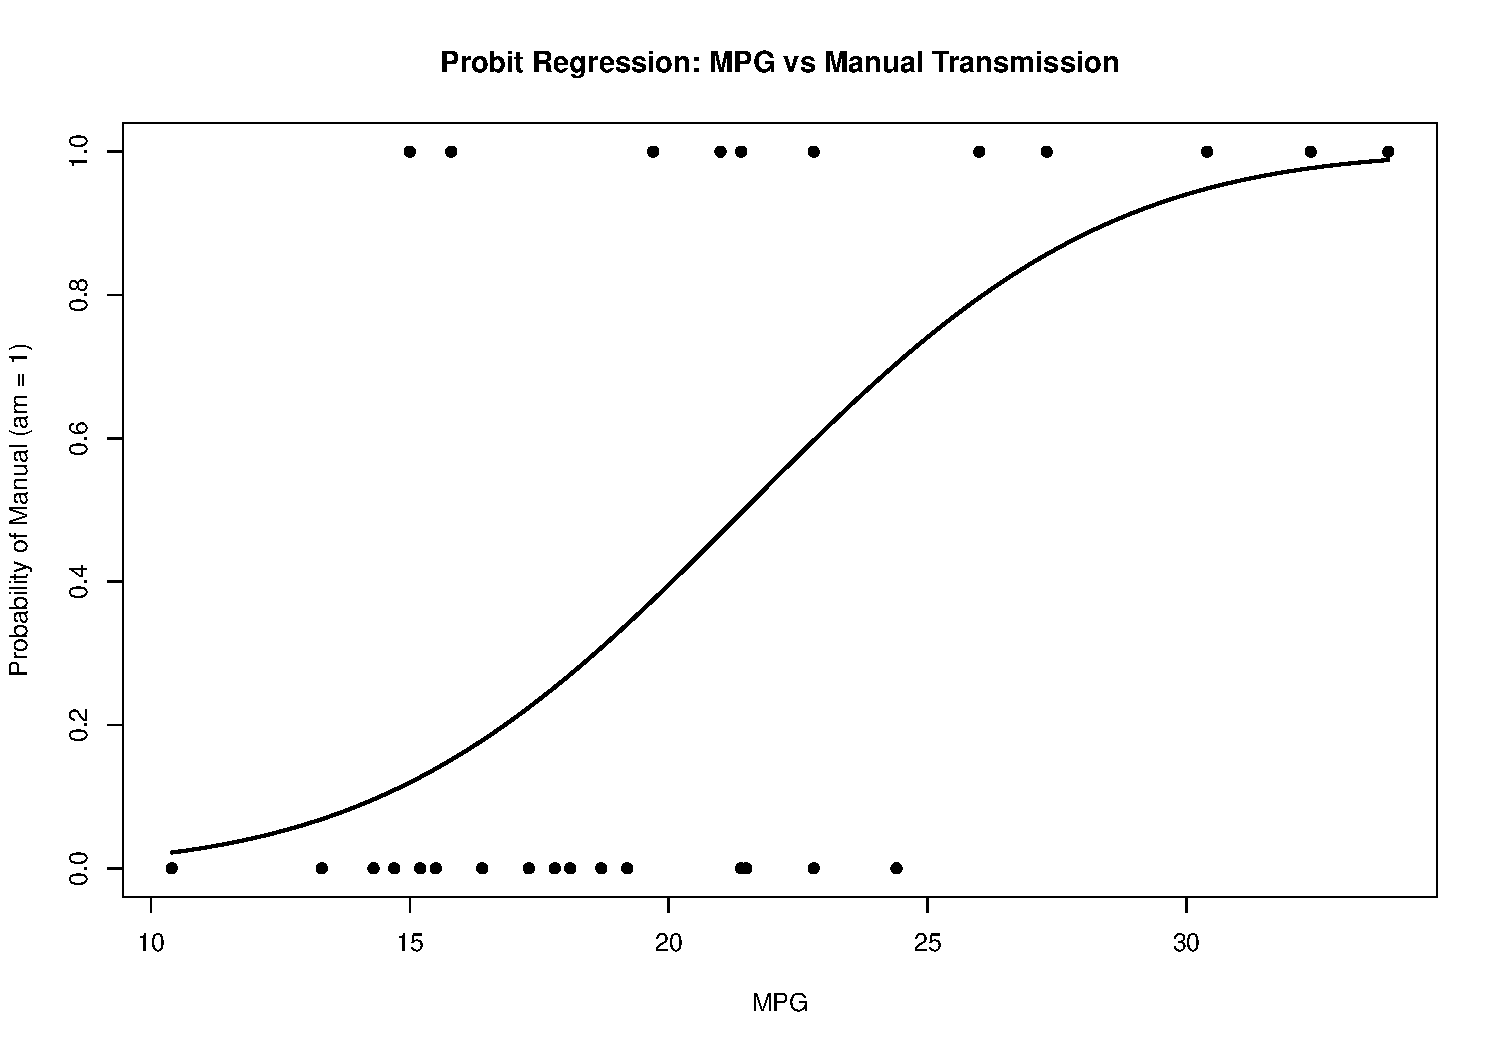
\includegraphics[keepaspectratio]{ProbitTheory_files/figure-beamer/unnamed-chunk-15-1.pdf}}

There is a positive relationship between MPG and the probability that a
car has a manual transmission: as fuel efficiency increases, the
likelihood that a car is manual increases.

\#New Slide

\begin{Shaded}
\begin{Highlighting}[]
\FunctionTok{library}\NormalTok{(margins)}
\NormalTok{mfx }\OtherTok{\textless{}{-}} \FunctionTok{margins}\NormalTok{(model)}
\FunctionTok{summary}\NormalTok{(mfx)}
\end{Highlighting}
\end{Shaded}

\begin{verbatim}
 factor    AME     SE      z      p  lower  upper
    mpg 0.0470 0.0080 5.8607 0.0000 0.0313 0.0628
\end{verbatim}

To answer our research question, what is the relationship between a
car's fuel efficiency (MPG) and the probability that it has a manual
transmission, for each 1 MPG increase, the probability that a car is
manual increases by about 4.7 percentage points (on average).\\

\#NewSlide
\end{block}

\begin{block}{Extension}
\protect\phantomsection\label{extension}
When extending the probit model to include multiple predictors, the
structure of the model remains unchanged:

\[
P(y=1) = \Phi(\beta_0 + \beta_1 \cdot \text{mpg} + \beta_2 \cdot \text{wt})
\]

Each coefficient represents a partial effect, meaning that the effect of
one variable is measured while holding the other variables constant.

If we add weight to the model, the MPG coefficient captures its effect
on transmission probability while holding weight constant---meaning it
reflects MPG's independent contribution rather than differences driven
by weight.

\#New Slide
\end{block}

\begin{block}{Government/Politics Dataset}
\protect\phantomsection\label{governmentpolitics-dataset}
\textbf{Research question}: to what extent do socioeconomic factors,
specifically age, education, and income, predict voter turnout in
American national elections?

We used a dataset provided by the American National Election Studies,
detailing whether individuals voted or not in the 2024 election. The
dataset had over 44 variables it considered, such as occupation and
religion.

\#New Slide

Translating information from the codebook, we considered the variables
below.

\begin{figure}
\centering
\pandocbounded{\includegraphics[keepaspectratio,alt={VCF0009z, considers if a survey accidentally talks to too many men and not enough women, the women's answers are given a higher weight (they count for more than one person) and the men's answers are given a lower weight (they count for less than one person).}]{images/clipboard-593014418.png}}
\caption{VCF0009z, considers if a survey accidentally talks to too many
men and not enough women, the women's answers are given a higher
\textbf{weight} (they count for more than one person) and the men's
answers are given a lower \textbf{weight} (they count for less than one
person).}
\end{figure}

We cleaned the dataset to only use the variables above

\#New Slide
\end{block}

\begin{block}{Exploratory Data Analysis}
\protect\phantomsection\label{exploratory-data-analysis}
\begin{Shaded}
\begin{Highlighting}[]
\FunctionTok{chisq.test}\NormalTok{(}\FunctionTok{table}\NormalTok{(df\_clean}\SpecialCharTok{$}\NormalTok{vote, df\_clean}\SpecialCharTok{$}\NormalTok{education))}
\end{Highlighting}
\end{Shaded}

\begin{verbatim}

    Pearson's Chi-squared test

data:  table(df_clean$vote, df_clean$education)
X-squared = 3910.4, df = 3, p-value < 2.2e-16
\end{verbatim}

\begin{Shaded}
\begin{Highlighting}[]
\FunctionTok{chisq.test}\NormalTok{(}\FunctionTok{table}\NormalTok{(df\_clean}\SpecialCharTok{$}\NormalTok{vote, df\_clean}\SpecialCharTok{$}\NormalTok{party\_id))}
\end{Highlighting}
\end{Shaded}

\begin{verbatim}

    Pearson's Chi-squared test

data:  table(df_clean$vote, df_clean$party_id)
X-squared = 3694.5, df = 6, p-value < 2.2e-16
\end{verbatim}

\begin{itemize}
\item
  For education, the test statistic is very large \(X^2 = 3910.4\) with
  a p-value effectively equal to zero. We can confidently reject the
  idea that voting behavior is independent of education level.
\item
  For party identification, the chi-squared test \(X^2 = 3694.5\) also
  produces a near-zero p-value, indicating a strong relationship between
  party ID and turnout.
\end{itemize}

\#New Slide

\begin{verbatim}
Warning in eval(family$initialize): non-integer #successes in a binomial glm!
\end{verbatim}

\begin{verbatim}

Call:
glm(formula = vote ~ age + education + income + party_id + interest, 
    family = binomial(link = "probit"), data = df_clean, weights = weight)

Coefficients:
                       Estimate Std. Error z value Pr(>|z|)    
(Intercept)          -1.2271752  0.0323903  -37.89   <2e-16 ***
age                   0.0145019  0.0003513   41.28   <2e-16 ***
educationHighSchool  -0.5935501  0.0171903  -34.53   <2e-16 ***
educationLessHS      -0.8753739  0.0229323  -38.17   <2e-16 ***
educationSomeCollege -0.2651494  0.0191872  -13.82   <2e-16 ***
income                0.1417566  0.0047471   29.86   <2e-16 ***
party_idIndLeanDem    0.3025451  0.0226679   13.35   <2e-16 ***
party_idIndLeanRep    0.3480854  0.0235716   14.77   <2e-16 ***
party_idStrongDem     0.6847337  0.0212788   32.18   <2e-16 ***
party_idStrongRep     0.7786772  0.0244692   31.82   <2e-16 ***
party_idWeakDem       0.3703462  0.0201312   18.40   <2e-16 ***
party_idWeakRep       0.4335910  0.0221265   19.60   <2e-16 ***
interest              0.4008260  0.0075930   52.79   <2e-16 ***
---
Signif. codes:  0 '***' 0.001 '**' 0.01 '*' 0.05 '.' 0.1 ' ' 1

(Dispersion parameter for binomial family taken to be 1)

    Null deviance: 74508  on 61812  degrees of freedom
Residual deviance: 61211  on 61800  degrees of freedom
AIC: 60653

Number of Fisher Scoring iterations: 4
\end{verbatim}

Latent scores.

\#New Slide

\begin{Shaded}
\begin{Highlighting}[]
\NormalTok{mfx }\OtherTok{\textless{}{-}} \FunctionTok{margins}\NormalTok{(model1)}
\FunctionTok{summary}\NormalTok{(mfx)}
\end{Highlighting}
\end{Shaded}

\begin{verbatim}
               factor     AME     SE        z      p   lower   upper
                  age  0.0039 0.0001  43.1511 0.0000  0.0037  0.0041
  educationHighSchool -0.1548 0.0041 -37.3483 0.0000 -0.1629 -0.1466
      educationLessHS -0.2449 0.0065 -37.5029 0.0000 -0.2577 -0.2321
 educationSomeCollege -0.0621 0.0044 -13.9750 0.0000 -0.0708 -0.0534
               income  0.0381 0.0013  30.1869 0.0000  0.0356  0.0405
             interest  0.1076 0.0019  56.2491 0.0000  0.1039  0.1114
   party_idIndLeanDem  0.0947 0.0071  13.3597 0.0000  0.0808  0.1086
   party_idIndLeanRep  0.1080 0.0073  14.8308 0.0000  0.0938  0.1223
    party_idStrongDem  0.1975 0.0063  31.4816 0.0000  0.1852  0.2098
    party_idStrongRep  0.2192 0.0068  32.4330 0.0000  0.2059  0.2324
      party_idWeakDem  0.1145 0.0063  18.1659 0.0000  0.1021  0.1268
      party_idWeakRep  0.1324 0.0068  19.5564 0.0000  0.1191  0.1456
\end{verbatim}

The average marginal effect (AME) of 0.0039 means that each additional
year of age increases the probability of voting by about \textbf{0.4
percentage points}, holding other factors constant. This suggests that
older individuals are more likely to vote.

Compared to individuals with a college degree (the baseline group),
those with lower levels of education are significantly less likely to
vote. For example, having only a high school education decreases the
probability of voting by about \textbf{15.5 percentage points}

The AME of 0.0381 shows that moving up one income category increases the
probability of voting by about \textbf{3.8 percentage points}.

Compared to independents, individuals who identify with a political
party, especially strong partisans, are substantially more likely to
vote. For example, strong Democrats and strong Republicans are about
\textbf{20--22 percentage points more likely} to vote than independents.

Similarly, \textbf{political interest} has one of the largest effects in
the model. The average marginal effect of 0.1076 indicates that moving
up one level of interest increases the probability of voting by about
\textbf{10.8 percentage points}.

Overall, while socioeconomic resources are important, these results show
that political engagement and partisan identity are equally powerful
predictors of turnout.
\end{block}
\end{frame}

\begin{frame}[fragile]{Appendix Code}
\protect\phantomsection\label{appendix-code}
\begin{Shaded}
\begin{Highlighting}[]
\NormalTok{model }\OtherTok{\textless{}{-}} \FunctionTok{glm}\NormalTok{(am }\SpecialCharTok{\textasciitilde{}}\NormalTok{ mpg, }
             \AttributeTok{data =}\NormalTok{ mtcars, }
             \AttributeTok{family =} \FunctionTok{binomial}\NormalTok{(}\AttributeTok{link =} \StringTok{"probit"}\NormalTok{))}

\NormalTok{mpg\_seq }\OtherTok{\textless{}{-}} \FunctionTok{seq}\NormalTok{(}\FunctionTok{min}\NormalTok{(mtcars}\SpecialCharTok{$}\NormalTok{mpg), }\FunctionTok{max}\NormalTok{(mtcars}\SpecialCharTok{$}\NormalTok{mpg), }\AttributeTok{length.out =} \DecValTok{100}\NormalTok{)}

\NormalTok{pred\_prob }\OtherTok{\textless{}{-}} \FunctionTok{predict}\NormalTok{(model, }\AttributeTok{newdata =} \FunctionTok{data.frame}\NormalTok{(}\AttributeTok{mpg =}\NormalTok{ mpg\_seq), }\AttributeTok{type =} \StringTok{"response"}\NormalTok{)}

\FunctionTok{plot}\NormalTok{(mtcars}\SpecialCharTok{$}\NormalTok{mpg, mtcars}\SpecialCharTok{$}\NormalTok{am,}
     \AttributeTok{xlab =} \StringTok{"MPG"}\NormalTok{,}
     \AttributeTok{ylab =} \StringTok{"Probability of Manual (am = 1)"}\NormalTok{,}
     \AttributeTok{main =} \StringTok{"Probit Regression: MPG vs Manual Transmission"}\NormalTok{,}
     \AttributeTok{pch =} \DecValTok{16}\NormalTok{)}

\FunctionTok{lines}\NormalTok{(mpg\_seq, pred\_prob, }\AttributeTok{lwd =} \DecValTok{2}\NormalTok{)}
\end{Highlighting}
\end{Shaded}

\begin{Shaded}
\begin{Highlighting}[]
\NormalTok{df }\OtherTok{\textless{}{-}} \FunctionTok{read.csv}\NormalTok{(}\StringTok{"anes\_timeseries\_cdf\_csv\_20260205.csv"}\NormalTok{, }\AttributeTok{stringsAsFactors =} \ConstantTok{FALSE}\NormalTok{)}


\NormalTok{vars }\OtherTok{\textless{}{-}} \FunctionTok{c}\NormalTok{(}\StringTok{"VCF0702"}\NormalTok{,  }\CommentTok{\# turnout}
          \StringTok{"VCF0101"}\NormalTok{,  }\CommentTok{\# age}
          \StringTok{"VCF0110"}\NormalTok{,  }\CommentTok{\# education}
          \StringTok{"VCF0114"}\NormalTok{,  }\CommentTok{\# income}
          \StringTok{"VCF0301"}\NormalTok{,  }\CommentTok{\# party ID}
          \StringTok{"VCF0310"}\NormalTok{,  }\CommentTok{\# political interest}
          \StringTok{"VCF0009z"}\NormalTok{) }\CommentTok{\# weights}

\NormalTok{df\_clean }\OtherTok{\textless{}{-}}\NormalTok{ df[, vars]}

\NormalTok{df\_clean[df\_clean }\SpecialCharTok{\textless{}} \DecValTok{0}\NormalTok{] }\OtherTok{\textless{}{-}} \ConstantTok{NA}

\CommentTok{\# Dependent Variable: Turnout (1 = voted, 0 = did not vote)}
\NormalTok{df\_clean}\SpecialCharTok{$}\NormalTok{vote }\OtherTok{\textless{}{-}} \FunctionTok{ifelse}\NormalTok{(df\_clean}\SpecialCharTok{$}\NormalTok{VCF0702 }\SpecialCharTok{==} \DecValTok{2}\NormalTok{, }\DecValTok{1}\NormalTok{,}
                  \FunctionTok{ifelse}\NormalTok{(df\_clean}\SpecialCharTok{$}\NormalTok{VCF0702 }\SpecialCharTok{==} \DecValTok{1}\NormalTok{, }\DecValTok{0}\NormalTok{, }\ConstantTok{NA}\NormalTok{))}

\NormalTok{df\_clean}\SpecialCharTok{$}\NormalTok{age }\OtherTok{\textless{}{-}} \FunctionTok{as.numeric}\NormalTok{(df\_clean}\SpecialCharTok{$}\NormalTok{VCF0101)}

\NormalTok{df\_clean}\SpecialCharTok{$}\NormalTok{education }\OtherTok{\textless{}{-}} \FunctionTok{factor}\NormalTok{(df\_clean}\SpecialCharTok{$}\NormalTok{VCF0110,}
                            \AttributeTok{levels =} \FunctionTok{c}\NormalTok{(}\DecValTok{4}\NormalTok{,}\DecValTok{3}\NormalTok{,}\DecValTok{2}\NormalTok{,}\DecValTok{1}\NormalTok{),}
                            \AttributeTok{labels =} \FunctionTok{c}\NormalTok{(}\StringTok{"CollegePlus"}\NormalTok{, }\StringTok{"SomeCollege"}\NormalTok{, }\StringTok{"HighSchool"}\NormalTok{, }\StringTok{"LessHS"}\NormalTok{))}

\NormalTok{df\_clean}\SpecialCharTok{$}\NormalTok{income }\OtherTok{\textless{}{-}} \FunctionTok{as.numeric}\NormalTok{(df\_clean}\SpecialCharTok{$}\NormalTok{VCF0114)}

\NormalTok{df\_clean}\SpecialCharTok{$}\NormalTok{party\_id }\OtherTok{\textless{}{-}} \FunctionTok{factor}\NormalTok{(df\_clean}\SpecialCharTok{$}\NormalTok{VCF0301,}
                           \AttributeTok{levels =} \FunctionTok{c}\NormalTok{(}\DecValTok{4}\NormalTok{,}\DecValTok{3}\NormalTok{,}\DecValTok{5}\NormalTok{,}\DecValTok{2}\NormalTok{,}\DecValTok{6}\NormalTok{,}\DecValTok{1}\NormalTok{,}\DecValTok{7}\NormalTok{),}
                           \AttributeTok{labels =} \FunctionTok{c}\NormalTok{(}\StringTok{"Independent"}\NormalTok{,}
                                      \StringTok{"IndLeanDem"}\NormalTok{,}
                                      \StringTok{"IndLeanRep"}\NormalTok{,}
                                      \StringTok{"WeakDem"}\NormalTok{,}
                                      \StringTok{"WeakRep"}\NormalTok{,}
                                      \StringTok{"StrongDem"}\NormalTok{,}
                                      \StringTok{"StrongRep"}\NormalTok{))}

\NormalTok{df\_clean}\SpecialCharTok{$}\NormalTok{interest }\OtherTok{\textless{}{-}} \FunctionTok{as.numeric}\NormalTok{(df\_clean}\SpecialCharTok{$}\NormalTok{VCF0310)}

\NormalTok{df\_clean}\SpecialCharTok{$}\NormalTok{weight }\OtherTok{\textless{}{-}}\NormalTok{ df\_clean}\SpecialCharTok{$}\NormalTok{VCF0009z}


\NormalTok{df\_clean }\OtherTok{\textless{}{-}} \FunctionTok{na.omit}\NormalTok{(df\_clean)}
\end{Highlighting}
\end{Shaded}

\begin{Shaded}
\begin{Highlighting}[]
\NormalTok{model }\OtherTok{\textless{}{-}} \FunctionTok{glm}\NormalTok{(am }\SpecialCharTok{\textasciitilde{}}\NormalTok{ mpg, }
             \AttributeTok{data =}\NormalTok{ mtcars, }
             \AttributeTok{family =} \FunctionTok{binomial}\NormalTok{(}\AttributeTok{link =} \StringTok{"probit"}\NormalTok{))}

\NormalTok{mpg\_seq }\OtherTok{\textless{}{-}} \FunctionTok{seq}\NormalTok{(}\FunctionTok{min}\NormalTok{(mtcars}\SpecialCharTok{$}\NormalTok{mpg), }\FunctionTok{max}\NormalTok{(mtcars}\SpecialCharTok{$}\NormalTok{mpg), }\AttributeTok{length.out =} \DecValTok{100}\NormalTok{)}

\NormalTok{pred\_prob }\OtherTok{\textless{}{-}} \FunctionTok{predict}\NormalTok{(model, }\AttributeTok{newdata =} \FunctionTok{data.frame}\NormalTok{(}\AttributeTok{mpg =}\NormalTok{ mpg\_seq), }\AttributeTok{type =} \StringTok{"response"}\NormalTok{)}

\FunctionTok{plot}\NormalTok{(mtcars}\SpecialCharTok{$}\NormalTok{mpg, mtcars}\SpecialCharTok{$}\NormalTok{am,}
     \AttributeTok{xlab =} \StringTok{"MPG"}\NormalTok{,}
     \AttributeTok{ylab =} \StringTok{"Probability of Manual (am = 1)"}\NormalTok{,}
     \AttributeTok{main =} \StringTok{"Probit Regression: MPG vs Manual Transmission"}\NormalTok{,}
     \AttributeTok{pch =} \DecValTok{16}\NormalTok{)}

\FunctionTok{lines}\NormalTok{(mpg\_seq, pred\_prob, }\AttributeTok{lwd =} \DecValTok{2}\NormalTok{)}
\end{Highlighting}
\end{Shaded}
\end{frame}

\end{document}
